% !TEX encoding = UTF-8
% !TEX TS-program = pdflatex
% !TEX root = ../tesi.tex

%**************************************************************
\chapter{Progettazione}
\label{cap:progettazione}
\label{sec:tecnologie-strumenti}

In questo capitolo vengono illustrate le strategie di progettazione adottate per la realizzazione del prodotto in questione. La progettazione viene descritta ad alto livello senza descrivere in dettaglio tutti i diagrammi delle classi. 

\section{Progettazione Frontend}
\label{sec:progettazione}
Come prima cosa sono stati realizzati utilizzando Figma i prototipi delle pagine da creare. In questo modo è stato possibile capire sin da subito la struttura delle pagina, rendendo cosi molto semplice la progettazione architetturale di tale pagine.
\subsection{Pagina cotenente l'editor}
Questa pagina contiene l'editor drag and drop. Per creare la struttura di questa pagina sono stati studiati diversi editor online che forniscono le stesse funzionalità(in diversi contesti). Dopo una attenta analisi delle strutture dei diversi editor online è stato concepita la seguente struttura:
\begin{figure}[!h] 
	\centering 
	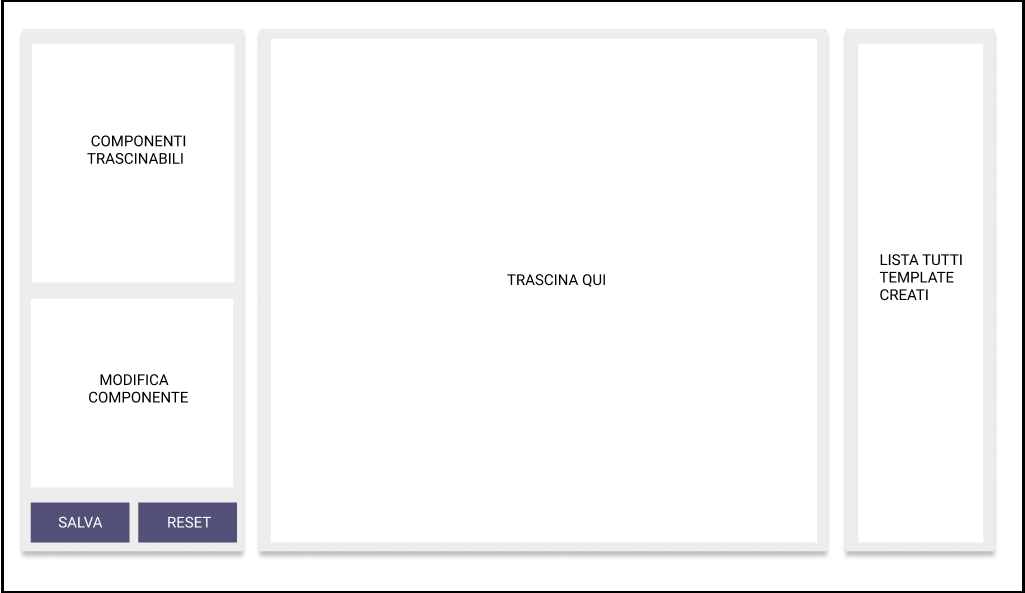
\includegraphics[width=0.9\columnwidth]{mock/mockeditor} 
	\caption{Mock pagina contenente l'editor}
\end{figure}  
\\
\begin{itemize}
	\item Il primo contenitore in alto a sinistra dovrà contenere tutti i componenti trascinabili. Ogni elemento rappresenta uno specifico tipo di oggetto HTML e CSS, come ad esempio il testo, banner, titolo, immagine ecc;
	\item Il secondo contenitore a sinistra contiene tutte le proprietà modificabili per ogni elemento;
	\item Il contenitore in centro rappresenta la zona dove tutti gli elementi vengono trascinati. In questo contenitore viene visualizzato a schermo il contenuto HTML e CSS contenuto in ogni elemento. Inoltre dovrà essere possibile modificare tale contenuto ed eliminare un elemento se necessario;
	\item Il contenitore a destra dovrà contenere tutti i template realizzati dagli utenti. Quindi esso contiene semplicemente una lista di tutti i template.  
\end{itemize}

\subsection{Pagina contenente il widget} Questa pagina contiene un semplice lista che dovrà contenere tutti i template da visualizzare nella pagina dei tickets, in modo che essa posono essere scelti dagli utenti da Zendesk.
\\ 
\subsection{Pagina login}
Semplice pagina contenete il form per il login. Una volta inseriti i valori validi l'utente sarà utenticato come amministratore, caricandoli cosi la pagina degli amministratore. 
\begin{figure}[!h] 
	\centering 
	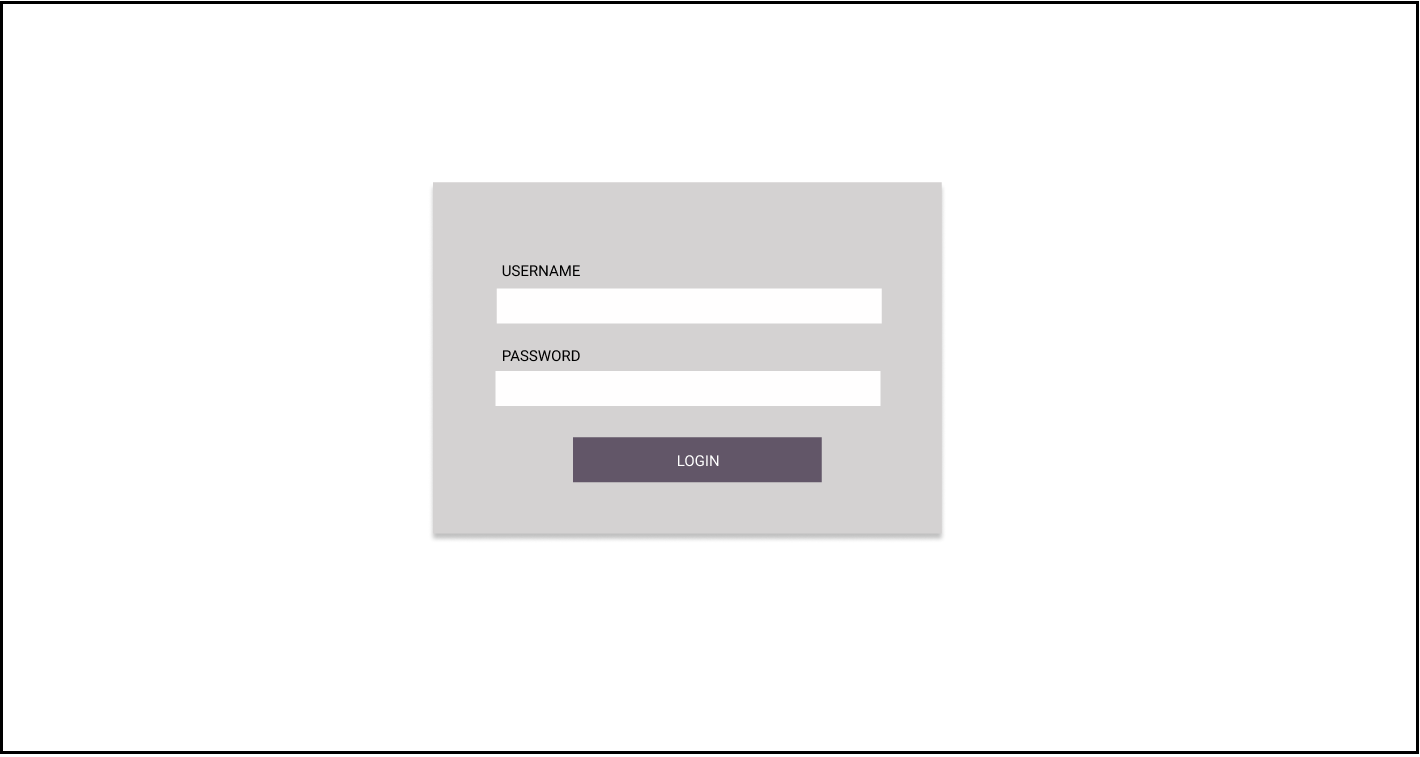
\includegraphics[width=1\columnwidth]{mock/mocklogin} 
	\caption{Mock pagina di login}
\end{figure}  \newpage
\subsection{Pagina degli amministratori}
Questa pagina dovrà essere realizzata per gli amministratore di Nextep, per permettere a loro di gestire tutti i clienti utilizzatore del applicazione. 
\begin{figure}[!h] 
	\centering 
	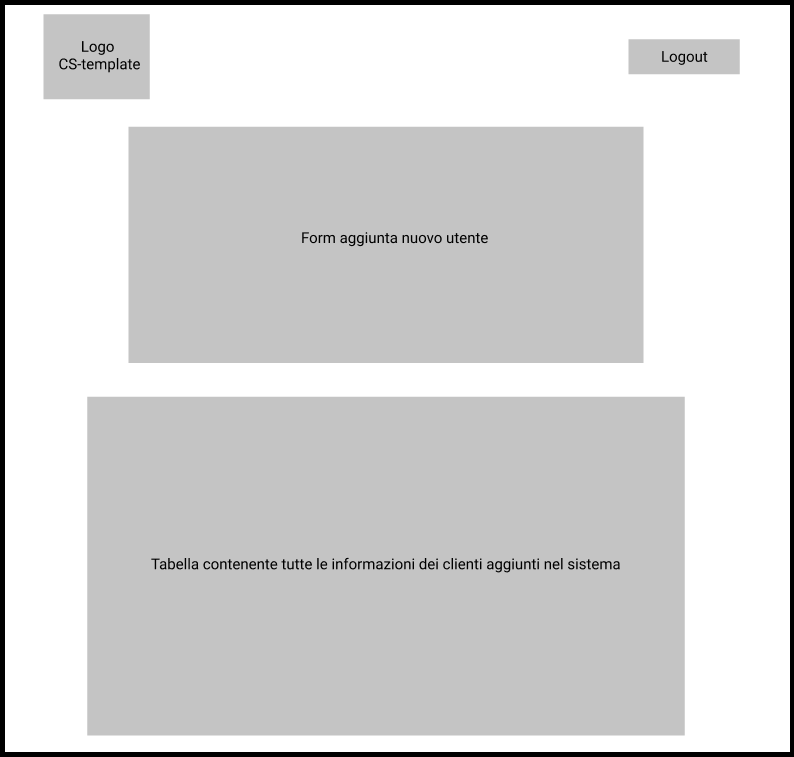
\includegraphics[width=0.8\columnwidth]{mock/mockadmin} 
	\caption{Mock pagina degli amministratori}
\end{figure}  
\begin{itemize}
	\item Contiene un semplice form per aggiungere un nuovo cliente;
	\item Contiene una semplice tabella, dove ogni elemento della tabella contiene le informazione di un singolo cliente.
\end{itemize}
\subsection{Atomic design}
Per realizzare le diverse pagine dell'applicazione è stato utilizzato il concetto di Atomic Design.
Creata da Brad Frost nel 2013, l'Atomic design è una metodologia composta da 5 differenti fasi, utile per creare un sistema di interfacce in maniera gerarchica. In questa metologia si parte dai componenti piu basilari possibili, fino ad arrivare alle pagine finali. Quindi è un approccio bottom-up.
\begin{figure}[!h] 
	\centering 
	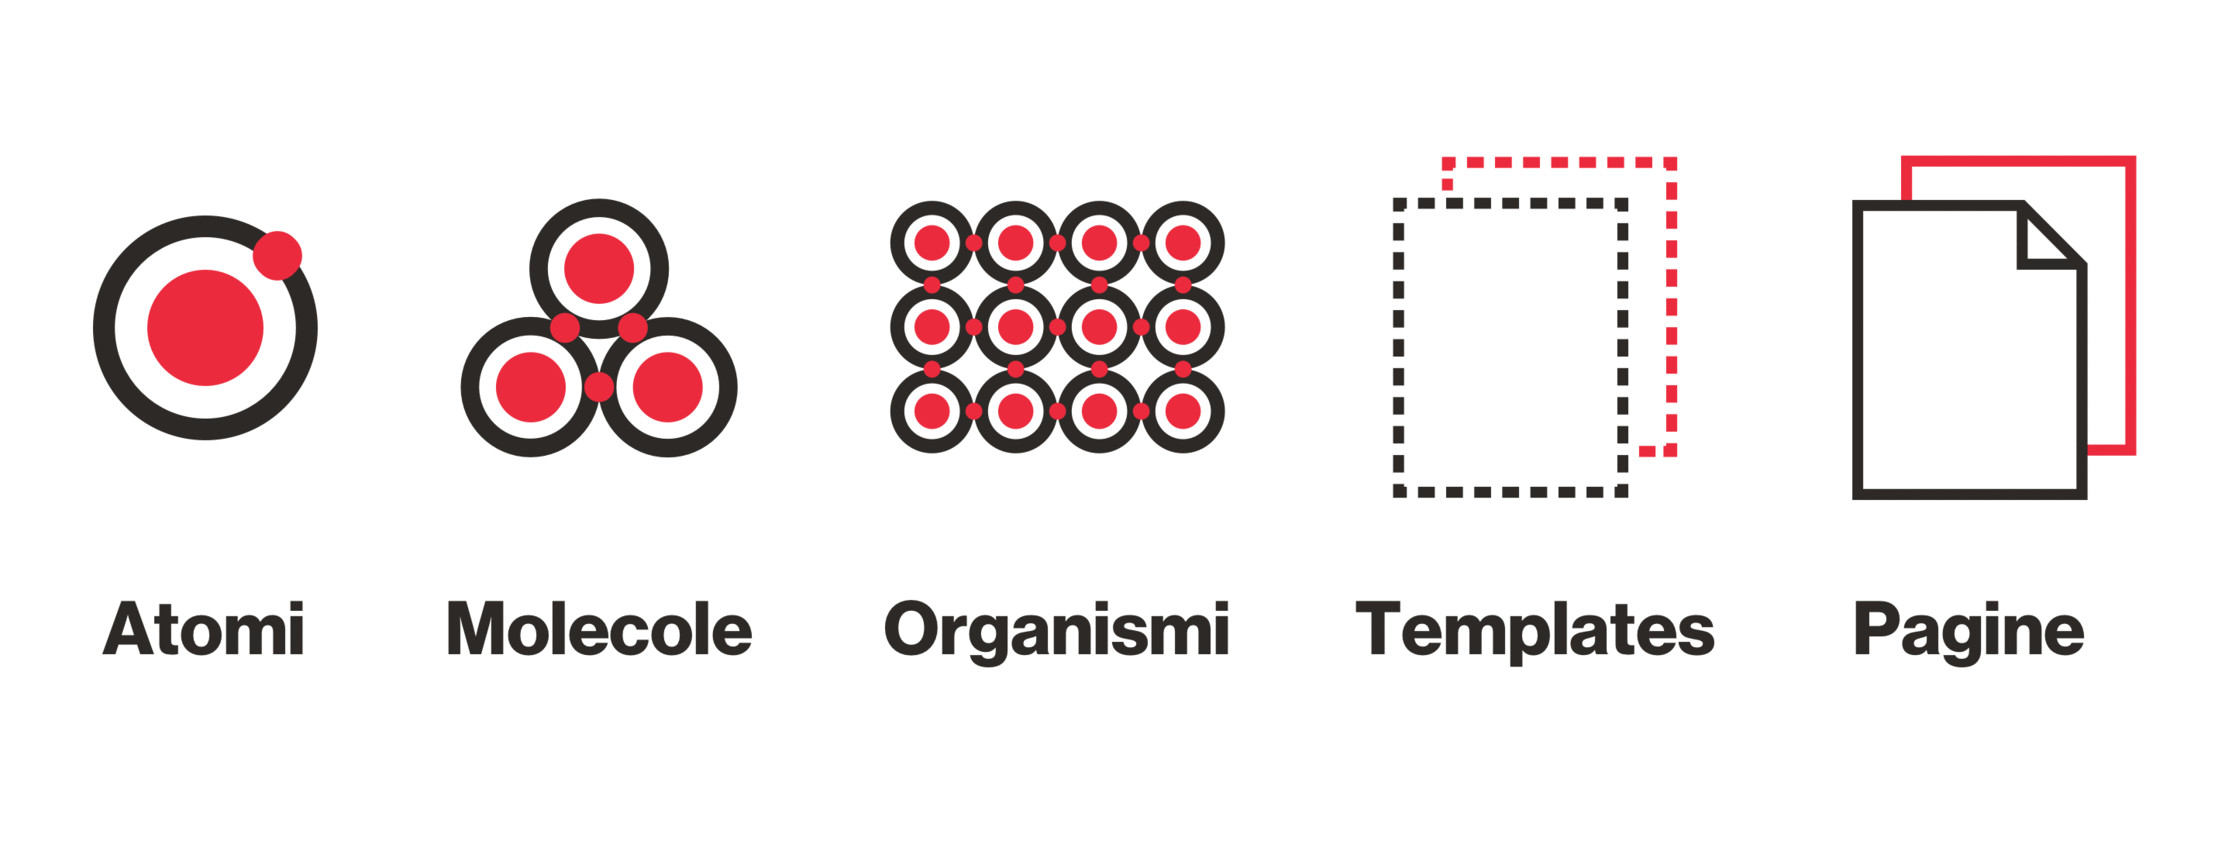
\includegraphics[width=0.8\columnwidth]{atomic} 
	\caption{Elementi atomic design}
\end{figure}
\\

\textbf{Atomi:} in fisica un atomo è la più piccola particella di un elemento che non subisce alterazioni nelle trasformazioni chimiche; nell’Atomic Design gli atomi sono i blocchi fondamentali che comprendono tutta l’interfaccia.
Questi atomi comprendono elementi HTML come tipografia, palette colori, input, bottoni e altri elementi che non possono essere suddivisi ulteriormente senza cessare di essere funzionali.
\\

\textbf{Molecole:} sono semplici gruppi di elementi d'interfaccia che funzionano uniti. Quando combiniamo due oppure più atomi, creiamo quindi una molecola.
\\

Nel contesto della applicazione gli atomi e le molecole sono rappresentate dai elementi della libreria Angular Material, che successivamente sono utilizzate per realizzare l'interfaccia di intera applicazione.

\begin{figure}[!h] 
	\centering 
	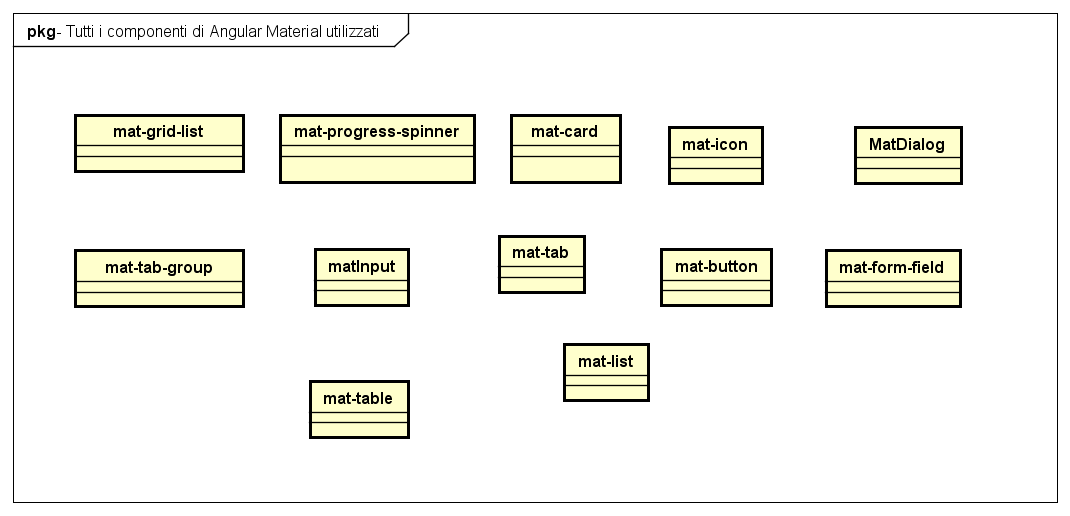
\includegraphics[width=1\columnwidth]{prog/angular} 
	\caption{Componenti Angular Material che formano gli atomi e le molecole dell'applicazione}
\end{figure} 

\textbf{Gli organismi:} sono dei componenti più o meno complessi, composti da gruppi di molecole e/o atomi e/o altri organismi. Questi organismi creano diverse sezioni all'interno della nostra interfaccia. Un esempio può essere un menu di navigazione, che è formato in media da diversi pulsanti/link. 
\\

\textbf{I templates:} sono creati dall'insieme dai nostri atomi, molecole e organismi. Creando così la prima idea di scheletro della pagina.
\\

\textbf{Le pagine:} sono dei templates riempiti di contenuto reale, come immagini, testi, elementi grafici, advertising, ecc. Questo ci aiuta a capire come la pagina, a seconda del caso specifico, si comporterà quando il contenuto andrà a popolarla. 
\subsubsection{Namespace 1} %**************************
Descrizione namespace 1.

\begin{namespacedesc}
    \classdesc{Classe 1}{Descrizione classe 1}
    \classdesc{Classe 2}{Descrizione classe 2}
\end{namespacedesc}


%**************************************************************
\section{Design Pattern utilizzati}

%**************************************************************
\section{Codifica}
